\begin{problem}{관광}
	{standard input}{standard output}
	{3 seconds}{256 megabytes}{}
	
	
	아름다운 자연관광을 가진 지구이웨의 왕 범수는, 지구이웨가 많은 관광객들을 유치해서 돈을 써 국고에 도움이 되어야 한다고 생각한다. 하지만 현실은 그의 꿈과는 멀다. 그래서 왕은 의원에게 문제를 조사하라고 하였다. 의원은 도로망이 제대로 갖춰있지 않아서 외국인들이 싫어한다는 사실을 알았다.
	
	지구이웨에는 $n$개의 마을이 있고, $m$개의 양방향 도로가 있으며, 도로가 서로 다른 두 말을을 잇는다. 도로들은 터널이나 고가도로가 있을 수 있다. 한 마을에서 도로를 통해서 다른 마을로 갈 수 있다는 보장은 없다.
	 
	의원은 현재의 도로망이 긴 여행에 적합하지 않다는 것을 알 수 있다. 어떤 사람이 여행을 시작하면, 같은 도시를 두번 지나지 않고서는 10개의 도시보다 많은 도시를 지날 수 없다.
	
	국고가 제한되어 있기 때문에, 새로운 도로를 지을 수는 없다. 하지만, 범수는 짧은 여행이 가능하다는것을 알리는 관광정보지점(Tourist Information Point, TIP)를 만들기로 했다. 모든 마을 마다, 그 마을 혹은 그 마을과 바로 인접한 마을에 TIP가 있어야 한다. 그리고, 어떤 마을에 TIP를 만드는 비용은 모든 마을마다 알려져 있다. 왕을 도와서 위의 조건을 만족하는 가장 저렴한게 TIP를 짓는 방법을 구하여라.
	
	\InputFile
	
	첫째 줄에는 지구이웨의 마을 수를 나타내는 $n$과 도로 수를 나타내는 $m$이 공백 하나로 구분되어 주어진다. ($2 \le n \le 20,000$, $0 \le m \le 25,000$) 마을은 1번부터 $n$번까지의 번호가 붙어있다. 입력의 둘째 줄은 $n$개의 정수 $c_1$, $c_2$, $\cdots$, $c_n$으로 이루어져 있고, $c_i$는 $i$번째 마을에 TIP를 짓는 비용을 나타낸다. 
	
	그리고 지구이웨의 도로망을 나타내는 정보가 주어진다. 다음 $m$개의 줄에는 두 정수 $a_i$, $b_i$ ($1 \le a_i < b_i \le n$)이 공백 하나로 구분되어 주어진다. 이것은 마을 $a_i$와 $b_i$가 도로로 연결되어있다는 것을 의미한다. 모든 두 마을 사이에는 최대 하나의 도로가 있다.
	
	\OutputFile
	첫째 줄에 TIP를 짓는 최소 비용을 정수 하나로 출력해야 한다.
	
	\SubtaskWithCost{1}{20}
	\begin{itemize}
		\item $n \le 20$
	\end{itemize}
	
	\SubtaskWithCost{2}{80}
	
	추가 제한조건이 없다.
	
	\Examples
		
	\begin{example}
	\exmp{
6 6
3 8 5 6 2 2
1 2
2 3
1 3
3 4
4 5
4 6

	}{%
7

	}%
	\end{example}
	
	\Note
	
	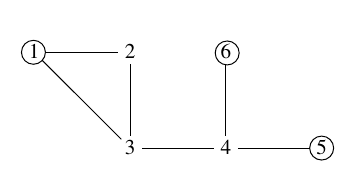
\includegraphics[]{tur.png}
	
	가장 저렴하게 TIP를 짓기 위해서는 1번, 5번, 6번 마을에 지어야 한다. (3+2+2=7 만큼의 돈이 든다.)
	
\end{problem}

